
\documentclass[a4paper,12pt,titlepage,final]{article}
% Language setting
% Replace `english' with e.g. `spanish' to change the document language
\usepackage[english, russian]{babel}

% Set page size and margins
% Replace `letterpaper' with `a4paper' for UK/EU standard size
\usepackage[letterpaper,top=2cm,bottom=2cm,left=3cm,right=3cm,marginparwidth=1.75cm]{geometry}
\usepackage{float}
% Useful packages
\usepackage{amsmath}
\usepackage{graphicx}
\usepackage[colorlinks=true, allcolors=blue]{hyperref}


\usepackage[T1,T2A]{fontenc}     % форматы шрифтов
\usepackage[utf8x]{inputenc}     % кодировка символов, используемая в данном файле
\usepackage{amsmath}      % для настройки размера полей
\usepackage{indentfirst}         % для отступа в первом абзаце секции
\begin{document}
\begin{titlepage}
    \begin{center}
    {\small \sc Московский Государственный Университет имени М. В. Ломоносова \\
    Факультет Вычислительной Математики и Кибернетики\\}
    \vfill
    
    {\large \bf Отчет по практическому заданию по курсу СКиПОД\\}
    \end{center}
    \begin{flushright}
    \vfill {
    Воробьев Евгений\\
    328 группа\\
    }
    \end{flushright}
    \begin{center}
    \vfill
    {\small Москва\\2022}
    \end{center}
    \par
\end{titlepage}

% Автоматически генерируем оглавление на отдельной странице
\tableofcontents

\newpage
\section{Цель}
Реализовать параллельную версию предложенного алгоритма с использованием технологий OpenMP и MPI.

\section{Предложенный алгоритм}\par
\subsection{Название}
Block Red-Black Ordering(Трехмерный)(\url{https://link.springer.com/article/10.1023/A:1021738303840})
\subsection{Описание}
Параллельное упорядочение называется «блочное красно-черное упорядочение». В этом методе узлы анализируемой сетки делятся на несколько или множество блоков, и к блокам применяется красно-черное упорядочение. Поскольку блоки с одинаковым цветом независимы друг от друга, прямые и обратные замены в итерации ICCG могут быть распараллелены для каждого цвета. Преимущество нового метода состоит в том, что в каждой параллельной подстановке существует только одна точка синхронизации. Для оценки сходимости и параллельного ускорения метода было проведено аналитическое исследование с использованием теории упорядочивающих графов и численных тестов на скалярном параллельном компьютере. Аналитическое исследование показывает, что скорость сходимости улучшается за счет увеличения количества узлов в одном блоке и что легко устанавливается оптимальный размер блока для получения наилучшей скорости сходимости. Численные тесты показывают, что новый метод обеспечивает высокую скорость параллельного ускорения благодаря быстрой сходимости, небольшим затратам на синхронизацию и эффективному использованию кэша данных на скалярном параллельном компьютере.
\newpage
\section{OpenMP}
\subsection{Изменение кода}
\begin{itemize}
\item Распараллелены вложенные циклы с помощью \textit{pragma omp parallel}
\item Добавлен замер времени с помощью \textit{omp\textunderscore get\textunderscore wtime()}
\end{itemize}
(код программы можно посмотреть на \url{https://github.com/user-vo2/-})
\subsection{Тестирование}
Запуск программы производлся для 1, 2, 4, 8, 32, 64 нитей по 4 раза. В таблицу записывалось среднее значение для каждого количества нитей.(здесь округлено до 3-х знаков после запятой)\par
\begin{tabular}{|c|c|c|c|c|c|c|c|}
\hline
	& 1 &	2 &	4 &	8 &	16 & 32 & 64\\
    \hline
150 &	5.766 & 3.598 & 2.827 &	1.989 &	1.538 &	0.954 &	0.723\\
    \hline
162 &	10.273 &	3.756 &	3.025 &	2.310 &	1.624 &	1.467 &	0.929\\
    \hline
200 &	19.698 &	12.830 &	6.606 &	3.456 &	2.733 &	2.383 &	1.943\\
    \hline
242 &	37.073 &	23.273 &	11.374 &	5.886 &	4.651 &	4.213 &	3.659\\
    \hline
258 &	83.225 &	62.334 &	37.765 &	24.446 &	17.514 &	14.574 &	7.746\\
    \hline
\end{tabular}
\par

\begin{figure}[h!]
  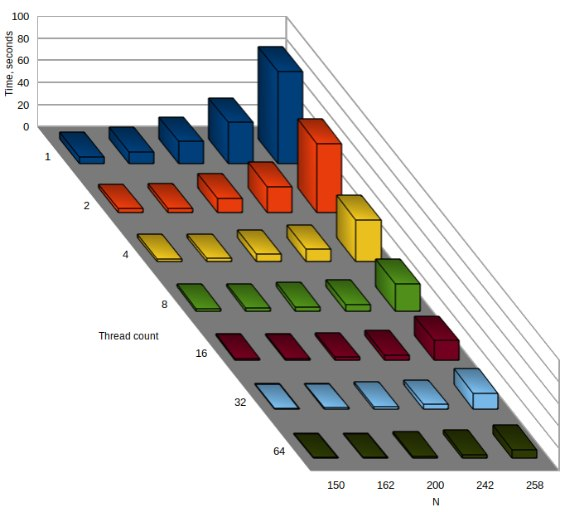
\includegraphics[width=0.7\linewidth]{omp_graph.jpeg}
  \caption{График для OMP}
  \label{fig:omp_graph}
\end{figure}
\newpage

\section{MPI}
\subsection{Изменение кода}
\begin{itemize}
\item Добавлено разделение матрицы по строкам в зависимости от количества процессов. Теперь каждый процесс обрабатывает только свою часть матрицы.
\item Реализованы функции \textit{pass\textunderscore first\textunderscore row()}, \textit{pass\textunderscore last\textunderscore row()} и \textit{wait\textunderscore all()} для взаимодействия процессов.
\item Добавлен замер времени с помощью \textit{MPI\textunderscore Wtime()}
\end{itemize}
(код программы можно посмотреть на \url{https://github.com/user-vo2/-})
\subsection{Тестирование}
Запуск программы производлся для 1, 2, 4, 8, 32, 64 процессов по 5 раз. В таблицу записывалось среднее значение для каждого количества процессов.(здесь округлено до 3-х знаков после запятой)\par
\begin{tabular}{|c|c|c|c|c|c|c|c|}
\hline
	& 1 &	2 &	4 &	8 &	16 & 32 & 64\\
    \hline
114 &	5.471 & 2.922 & 1.639 &	0.968 &	0.651 &	0.582 &	1.384\\
    \hline
130 &	8.491 &	4.313 &	2.215 &	1.194 &	0.842 &	0.859 &	2.169\\
    \hline
162 &	15.834 &	8.021 &	4.067 &	2.133 &	1.363 &	1.472 &	4.035\\
    \hline
242 &	55.071 &	27.765 &	14.034 &	7.259 &	4.298 &	4.301 &	14.056\\
    \hline
258 &	73.385 &	36.965 &	18.719 &	9.799 &	5.502 &	5.981 &	18.619\\
    \hline
\end{tabular}
\par

\begin{figure}[h!]
  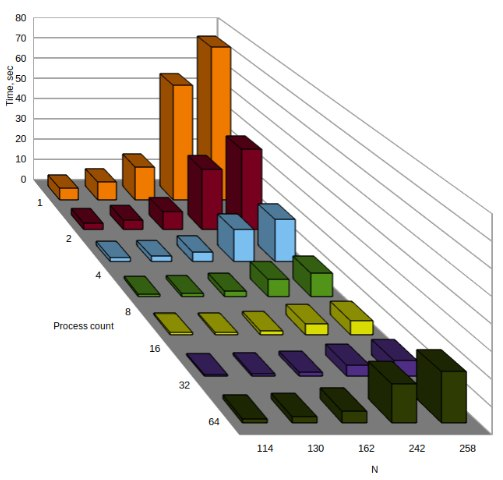
\includegraphics[width=0.6\linewidth]{mpi_graph.jpeg}
  \caption{График для MPI}
  \label{fig:mpi_graph}
\end{figure}
\newpage

\section{Вывод}
Выполнена работа по разработке параллельной версии алгоритма (Red-Black Ordering 3D). Изучены
технологии написания параллельных алгоритмов OpenMP и MPI. Проанализировано время выполнения
алгоритмов на различных вычислительных системах.\par
Технология OpenMP удобна в использовании, причем дает значительный прирост производительности на
рассчитанных на многопоточные вычисления системах.\par
MPI можно назвать более низкоуровневой технологией: разработка MPI-программы знакомит с основами
взаимодействия вычислительных узлов суперкомпьютера.\par
В общем зачете OpenMP показала лучшие результаты чем MPI. Это связано с накладными расходами на распараллеливание.
\section{Ссылки}
\begin{raggedright}
\begin{itemize}
\item \url{https://github.com/user-vo2/-}
\item \url{https://link.springer.com/article/10.1023/A:1021738303840}
\end{itemize}
\end{raggedright}
\end{document}